\centerline{\bf \Huge  Матдрака 2}

\begin{flushright}
    \scriptsize Ну и молодёжь пошла! Ты ему в морду, а он сразу в драку.\\ Кенпачи Зараки
\end{flushright}

\problem{1} Найдите все пары простых чисел, разность квадратов которых является простым числом. Ответ обоснуйте.
%(3, 2)

\problem{2}Из книги выпал кусок, страницы которого имеют номера от 480 до 612. Сколько страниц в выпавшем куске?
%132

\problem{3}Петя задумал число, которое сначала уменьшил на 7, затем уменьшил в 10 раз и получил результат, который на 34 меньше исходного. Какое число задумал Петя?
%37

\problem{4}Найдите сумму цифр в десятичной записи числа $4^{13}\cdot5^{21}$.
%32

\problem{5}Найдите $x^3 + y^3$, если известно, что $x + y = 5 \ \text{и} \ x + y + x^2y + xy^2 = 24.$
%68

\problem{6}Найдите наименьшее число, кратное 45, десятичная запись которого состоит только из единиц и нулей.
%1111111110

\problem{7}Найдите наименьшее натуральное значение n, при котором число $n!$ делится на $990$.
%11

\problem{8}Шахматист сыграл в турнире 20 партий и набрал 12,5 очков. На сколько партий больше он выиграл, чем проиграл?
%5

\begin{wrapfigure}{r}{0.15\textwidth}
\centering
    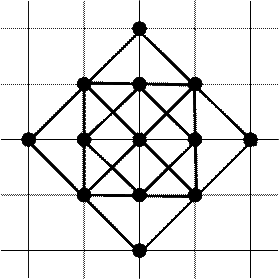
\includegraphics[width=0.15\textwidth]{Сборы/Сборы Элиста 2023/fightpict.png}
\end{wrapfigure}

\problem{9}На рисунке изображено 13 точек. Сколько квадратов с вершинами в этих точках можно нарисовать? (Точки располагаются все в вершинах квадратиков со стороной 1)
%11

\problem{10}. Сколько существует пятизначных чисел, десятичная запись которых начинается с 1 и содержит ровно две одинаковые цифры?
%5040

\problem{11}Сколькими способами можно расставить числа 1 и -1 во всех клетках таблицы $4 \times 4$ так, чтобы сумма всех чисел в каждой строке и в каждом столбце была равна 0?
%90

\problem{12}Найдите наименьшее натуральное n такое, что все 73 дроби $\dfrac{19}{n+21}, \ \dfrac{20}{n+22}, \ \dfrac{21}{n+23}, 
 \dotsc,\\ 
\dfrac{91}{n+93}$ несократимы.
%95

\newpage

\hspace{3mm}

\problem{13}В каждой клетке квадрата 3×3 лежит монета орлом вверх. Какое наименьшее количество монет нужно перевернуть, чтобы в результате не оказалось трех монет, расположенных в одной вертикали, одной горизонтали или одной диагонали и лежащих одинаково (то есть все три орлом вверх или все три решкой вверх)?
%4

\problem{14}Расположите в порядке возрастания числа: $222^2; 22^{22}; 2^{222}; 22^{2^{2}}; 2^{22^2}; 2^{2^{22}}; 2^{2^{2^2}}$. В ответе запишите число по типу 2134647
%1742356


\problem{15}Существует ли треугольник, градусная мера каждого угла которого выражается простым числом? Если да, то в ответ запишите, какие у него углы.

\problem{16}Найдите наибольшее натуральное n, при котором  $n^{200} < 5^{300}$.
%11

\problem{17}Герман спускался по лестнице из своей квартиры к другу Глебу, который живет на первом этаже. Когда он спустился на несколько этажей, оказалось, что он прошёл треть пути. Когда он спустился ещё на один этаж, ему осталось пройти половину пути. На каком этаже живёт Герман?
%7

\problem{18}Алина пишет подряд натуральные числа: 123456789101112... .
На каких местах, считая от начала, в первый раз будут стоять три цифры 5 подряд?
%100, 101, 102

\problem{19}Алина вступила в битву против НеНачальника, бросив ему вызов в покере. Раскрыв сущность своего стенда Osirius, она научилась со стопроцентной вероятностью тасовать себе в руку две пары и любую другую карту. Сколькими способами стенд Алины может положить в ее руку две пары и любую карту из оставшихся?
%3744

\problem{20}Треугольная числовая таблица построена таким образом: в вершине, составляющей нулевую строчку, стоит число 0, в n–й строчке на левом и правом концах стоит по числу n, и между каждыми двумя соседними числами n–ой строчки в (n+1)–ой стоит их сумма. Найдите сумму всех чисел в сотой строчке.
%2^101 - 1 